%* what is known
Localized surface plasmon resonance (LSPR) is an optical effect where an 
electromagnetic wave excites the free electrons on the surface of a metallic nanoparticle.
These vibrations of the electron cloud are known as plasmons, and in LSPR they resonate with the incoming
field (see Figure \ref{fig:lspr}). When this happens, most of the incoming energy
is either absorbed by the nanoparticle, or scattered in different directions,
generating a large shadow behind the scatterer (extinction). In the case of LSPR,
the wavelength of the incoming wave is usually considered to be much larger than 
the size of the nanoparticle.

This principle is used to design 
biosensors, as the resonance frequency is highly dependent of the dielectric environment 
around the scatterer. 
Then, the resonance frequency shifts when an analyte binds to the nanoparticle, 
resulting in a very sensitive sensor \cite{HaesETal2004, HaesVanduyne2002}.

A number of researchers have used numerical simulations to study LSPR \cite{SolisTaboadaObelleiroLiz-MaarzanGarciadeabajo2014}. These mostly rely on the 
solution of Maxwell's equations in some form, solved by means of finite difference time-domain (FDTD),
boundary element, or finite element methods. 
These simulations have been used to study the 
optical properties of dielectric or metallic nanoparticles \cite{Hohenester2018,HohenesterTrugler2012,
JungPedersenSondergaardPedersenLarsenNielsen2010, VideenSun2003,
MayergoyzFredkinZhang2005, MayergoyzZhang2007}, interactions between nanoparticles
and electron beams \cite{GarciadeabajoAizpurua1997, GarciadeabajoHowie2002},
and surface plasmon resonance sensors.
Among the latter application we find biosensors, where researchers have modelled the 
interaction between the metallic nanoparticle and target molecules with highly 
simplified methods \cite{JungCampbellChinowskyMarYee1998,HaesVanduyne2002,DavisGomezVernon2010,AntosiewiczApellClaudioKall2011}.

\begin{figure}[h] %  figure placement: here, top, bottom, or page
   \centering
   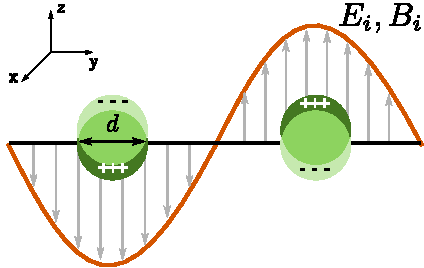
\includegraphics[width=0.35\textwidth]{lspr.pdf} 
   \caption{Localized Surface Plasmon Resonance (LSPR) scheme. }
   \label{fig:lspr}
\end{figure}

%* What is unknown, limitations and gaps

In the biosensor community most progress is achieved 
through experimental analysis, with trial and error procedures {\color{blue} I also have this impression, but do we have a reference to support it? If not, I'd rather avoid it}. 
Using software to assist the design process can play a key role for the manufacture and optimization
of biosensors, as we have access to details that are not available in experimental tests.
For example, empirical studies suggest that the sensitivity of the sensor
is highly dependent on the distance between the nanoparticle and the analyte \cite{HaesETal2004};
these results were modeled with a simplified discrete dipole approximation (DDA), however, 
the analyte was not considered in the analysis. Moreover, experiments show that 
LSPR sensors are sensitive enough to detect conformational changes of the analytes \cite{HallETal2011}, 
but current simplified models of LSPR are not able to consider such details.

%* Fill the gap

Even though LSPR is an optical effect, electrostatics 
makes a good approximation in the long-wavelength limit. In this work we use
the boundary integral electrostatics solver \pygbe \cite{CooperETal2016} 
to compute the extinction cross-section of metallic nanoparticles, and study how LSPR 
response changes in the presence
of a biomolecule. \pygbe was recently extended to account for complex dielectric constants 
\cite{ClementiETal2017} aiming towards the LSPR biosensing application. We treat Maxwell's
equations quasi-statically \cite{MayergoyzZhang2007} and
use an accurate continuum representation of the biomolecule obtained from the
crystal structure. 

The boundary element solver in \pygbe
is accelerated with a treecode (an $\mathcal{O}(N\log N)$ fast solver), and runs on
graphic processing units (GPUs). Also, the software
\footnote{\url{https://github.com/barbagroup/pygbe}} is shared under the 
BSD 3-clause license and the development repository is available on Github.


%{\color{red}  Keeping this structure here for reference until we polish better
%the introduction.

%What is known:
%\begin{itemize}
%\item Plasmonic simulations, what applications they cover, etc. (cite Matlab guy, also Garcia de Abajo, Jung+Pedersen, etc. Maybe we can even cite COMSOL here)
%\item LSPR: how does it work, what simulations are there in the literature. Talk about work from, for example, Davis or van Duyne. See page 50 of my thesis (end chapter 2).
%\end{itemize}

%What is unkown:
%\begin{itemize}
%\item all developments are trial and error
%\item no computational tools to help in the design process
%\item example: no understanding of the sensitivity of the system
%\item models that consider the nanoparticle and the analyte are extremely simplistic
%\end{itemize}

%Fill the gap:
%\begin{itemize}
%item design of a computational tool that is highly accurate to represent the biomolecule
%\end{itemize}
%}

